\section{Système complet: processeur et mémoires}

Le système complet, ou top module, instancie une Quadram décrite en VHDL et le processeur décrit en Verilog. Le top module a une horloge et le signal de reset en logique négative et en sortie, le bus de données. 
Son comportement est décrit en VHDL; un composant est défini pour faire appel au module \textit{simple\_proc} correspondant au processeur.
Pour conserver la générécité, il est possible de définir la taille du bus de données et du bus d'adresses, ainsi que le nombre de bits de poids fort à isoler pour le décodeur d'adresses. \\

\subsection{Simulation}

\indent Via Modelsim, il est possible de charger des valeurs hexadécimales dans la mémoire \textit{MEM} du processeur: ces valeurs sur 4 octets sont des instructions définies dans le jeu d'instructions du processeur.
En simulation, à chaque coup d'horloge, une instruction est chargée, décodée et executée. L'exécution séquentielle de ces instructions permet de tester le fonctionnement global du système.
L'approche choisie est de stocker des valeurs \textit{immediate} contenue dans un champs de l'instruction \textit{Store} en mémoire puis de charger ces valeurs dans les registres tampons du processeur.
Pour le test, des opérations mathématiques sont effectuées sur ces valeurs: une addition puis une multiplication, le tout en faisant intervenir différentes cellules \gls{RAM} de la mémoire.
Pour les tests, les paramètres ont été définis de la façon suivante:

\begin{equation}
	\notag
	 \begin{cases}
		ABUS SIZE = 10 & \\
		DBUS SIZE = 32 & \\
		NB MSB = 2
	\end{cases}
\end{equation}

\begin{figure}[h]
	\centering
	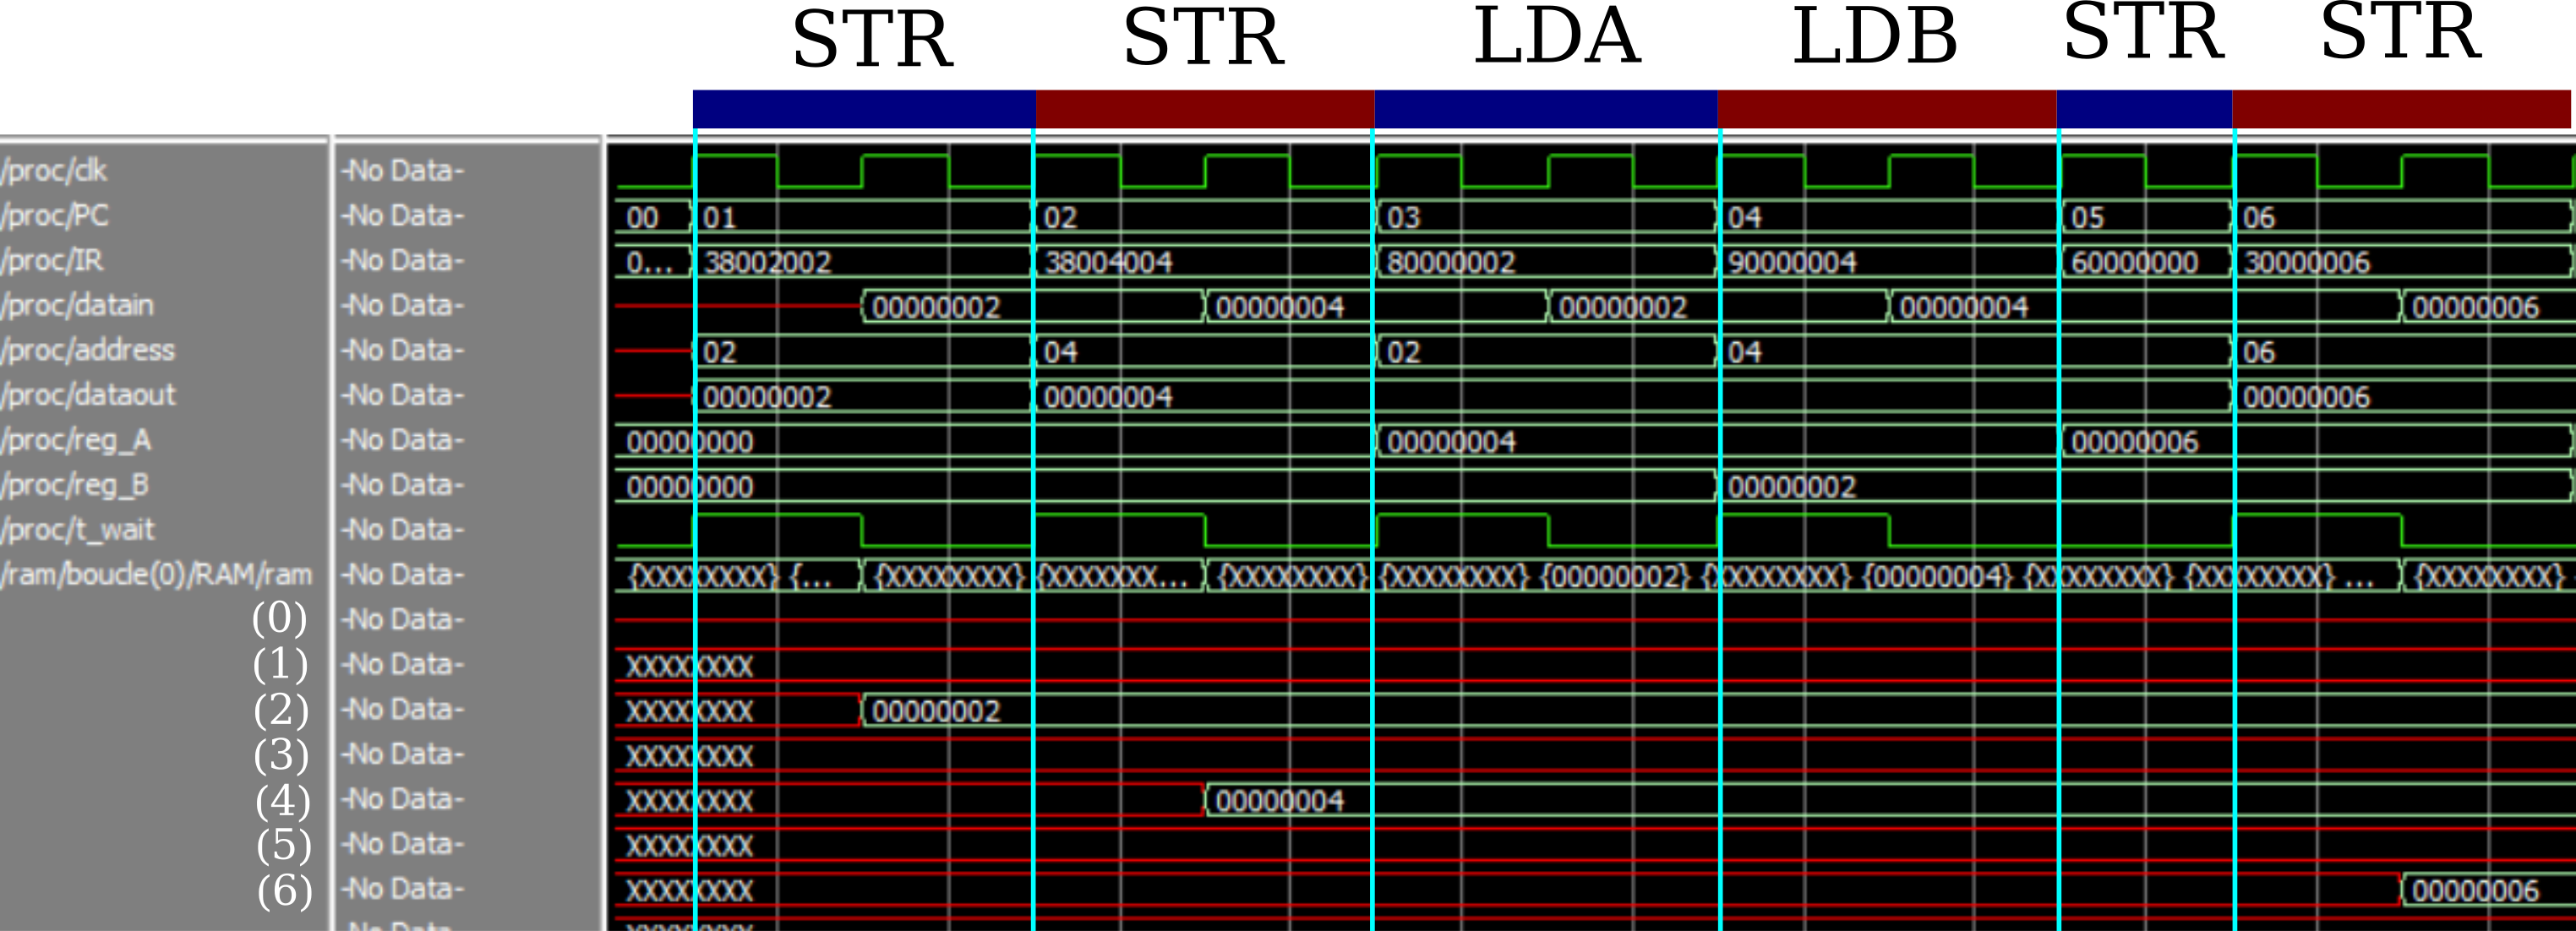
\includegraphics[width=0.97\linewidth]{top_ram_add.draw.png}
	\caption{Simulation du top module}
	\label{fig:wave_top_module}
\end{figure}

\indent Ce chronogramme correspond aux instructions executées pour obtenir le résultat de l'addition 2 + 4 en mémoire.
Nous pouvons observer les deux coups d'horloge nécessaires pour les instructions \textit{Load} et \textit{Store}, permis par l'activation du signal \textit{wait}.
En mémoire, les valeurs apparaissent de manière séquentielle au fur et à mesure que les instructions s'exécutent.
Le résultat attendu (2 + 4 = 6) est retrouvé en mémoire à l'adresse souhaitée.
Dans le cas du test ci-dessus, une seule mémoire est sollicitée. 
D'autres tests ont été effectués et valident le comportement du système pour une multiplication de deux valeurs contenues dans des mémoires différentes.
Ci-dessous le fichier .txt des instructions chargées en mémoire.

\newpage

\begin{lstlisting}[frame=single, basicstyle = \ttfamily \footnotesize]
	38002002 // STR immediate value 2 at address 2 (ram 0)	
	38004004 // STR immediate value 4 at address 4 (ram 0)
	80000002 // LDA value from address 2
	90000004 // LDB value from address 4
	60000000 // ADD values from registers A and B
	30000006 // STR value from register A at address 6 (ram 0)
	38003003 // STR immediate value 3 at address 3 (ram 0)
	38005084 // STR immediate value 5 at address 4 (ram 2)
	80000003 // LDA value from address 3
	90000084 // LDB value from address 4
	70000000 // MUL values from registers A and B
	30000086 // STR value from register A at address 6 (ram 2)
	00000000 // HLT
\end{lstlisting}

\subsection{Analyse RTL du module}

\indent Tout au long du rapports, des blocs au niveau \gls{RTL} des différents blocs ont été utilisé à des fins d'illustration.
Ces blocs étaient issus de la synthèse du top module réalisée sous Vivado.
Pour synthétiser le sytème, il a fallu retirer certains éléments non synthétisables du processeur notamment les commandes \textit{step} qui ajoutaient un offset de 10 ns ou encore les commandes ModelSim.

\begin{figure}[h]
	\centering
	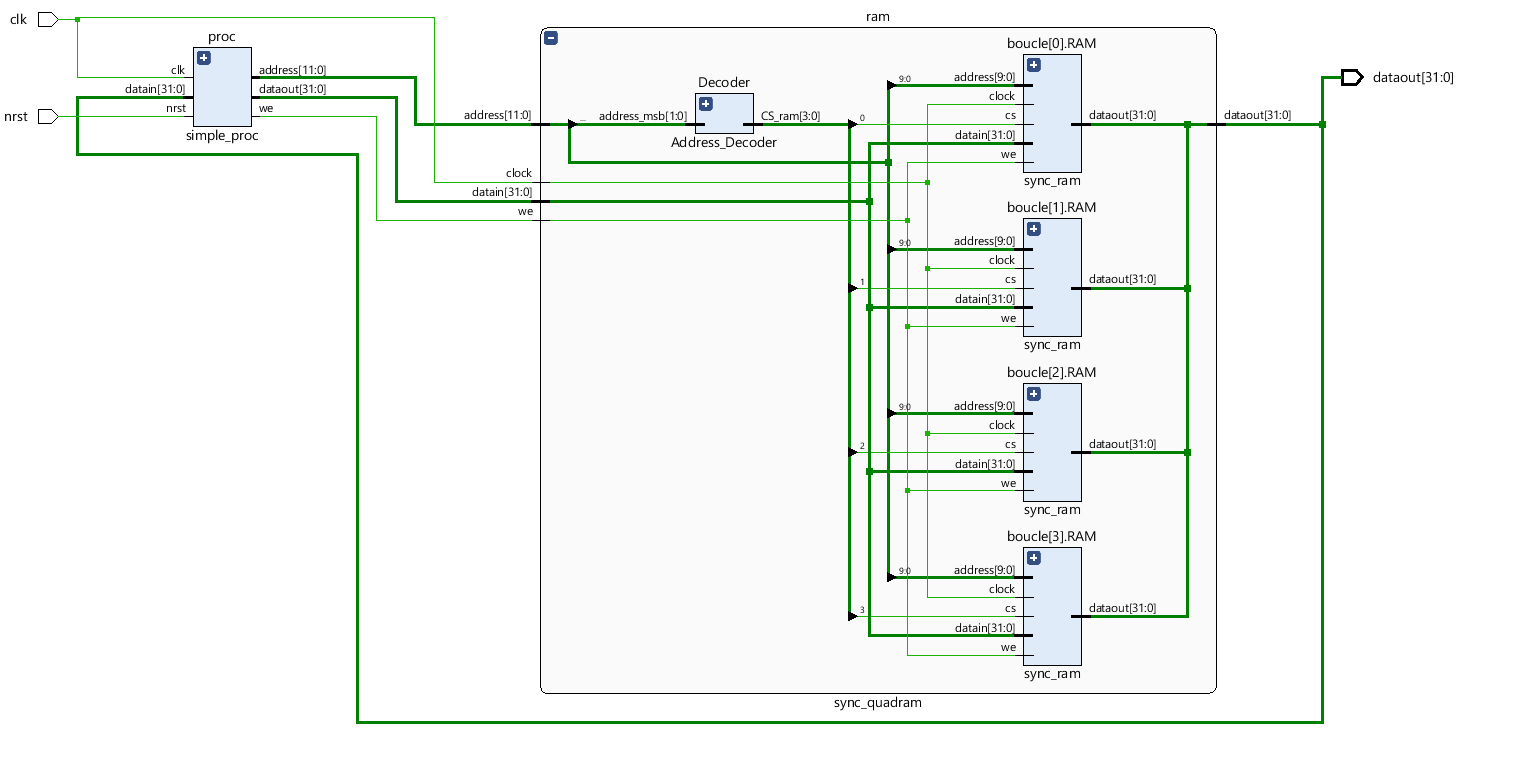
\includegraphics[width=0.97\linewidth]{synth_top_module.png}
	\caption{Synthèse du top module}
	\label{fig:synth_top_module}
\end{figure}


